\documentclass[12pt]{article}
\usepackage[margin=1in]{geometry}
\usepackage{amsmath,amssymb,amsthm,mathtools}
\usepackage[T1]{fontenc}
\usepackage[utf8]{inputenc}
\usepackage{lmodern}
\usepackage{microtype}
\usepackage{xcolor}
\usepackage{hyperref}
\hypersetup{colorlinks=true,linkcolor=blue,urlcolor=blue,citecolor=blue}
\setlength{\parindent}{0pt}
\setlength{\parskip}{0.75em}
\newtheorem{theorem}{Theorem}
\newtheorem{proposition}{Proposition}
\newtheorem{corollary}{Corollary}
\newtheorem*{remark}{Remark}
\newcommand{\E}{\mathbb{E}}
\newcommand{\IM}{\mathrm{IM}}
\usepackage{lettrine}
\usepackage{fancyhdr}
\usepackage{authblk}

\pagestyle{fancy}
\fancyhf{} % clear all header and footer fields
\fancyhead[R]{Revenue or Resilience? \thepage} % Right side header
\fancyhead[L]{Andrew Wang}       % Left side header (page number)

\author[1]{Andrew Wang}
\affil[1]{University of Washington}

\title{Revenue or Resilience? Evidence from a Regional Windfall in China}

\usepackage{biblatex}
\addbibresource{references.bib}

\begin{document}
\maketitle

\begin{abstract}
Why do states provide public goods? The existing literature generally provides revenue-maximizing explanations: the provision of public goods increases long-term revenue gains by improving market performance and by reducing the costly coercion required to generate revenue. I argue, however, that existing revenue-maximizing models belie a revenue-resilience tradeoff; states provide public goods to balance revenue and resilience. I identify one state (China) that should find net utility in the provision of public goods itself, \textit{sans} any revenue effects. This problem is difficult to verify because a stationary revenue-maximizing state may behave identically to a resilience-maximizing state if the revenue spike is long-term, if it is dispersed, or if existing state capacity in the affected region is weak. I identify an exogenous, short-term, localized growth in a region with strong public goods provision: Inner Mongolia's economic boom following Chinese export restrictions on Rare Earth Elements from 2010-2011. In this case, I find that China's national government was not revenue maximizing but jointly revenue- and resilience- maximizing.
\end{abstract}

\section{Introduction}

\lettrine[]{W}{hy} do states provide public goods? Existing political economy explanations generally treat public goods provision as part of a revenue-maximizing strategy: states invest in public goods because doing so improves long-run extraction by increasing economic productivity and reducing the coercive cost of generating revenue. In this view, rulers seek revenue subject to constraints imposed by bargaining power, institutional design, and the transaction costs of enforcement \parencite{levi1988}. On the other hand, public goods improve market performance, strengthen state capacity, and encourage quasi-voluntary compliance by making taxation appear fairer and more predictable.

Raising the tax rate increases revenue initially, but beyond that point reduces productivity and compliance because of the increasing transaction costs of enforcing the tax rate, raising the cost of extraction. Levi shows that public goods enable a higher tax rate and hence a higher maximum revenue by increasing productive output and reducing enforcement costs. I argue, however, that public goods may also be valued to preserve resilience, defined here as the governing slack that remains before coercive demands become politically costly or institutionally destabilizing. In that sense, expenditure on public goods is useful even where its marginal return to revenue is low if it lowers the coercive cost required to maintain stability.

This logic explains why states often provide public goods even when doing so reduces short-run net revenue, yet it leaves open a broader question: do states invest in public goods only because they improve extraction, or also because they reduce the coercive burden of governing even when marginal revenue returns to this investment are low? I begin by asking a prerequisite question: if additional expenditure yields relatively little gain in future revenue but preserves coercive slack in a sensitive region, should a revenue-maximizing state still spend there?

To evaluate this question, I formalize a revenue-maximizing state constrained by coercive feasibility and then provide a model of a state that jointly values revenue and resilience. I construct this model such that the state chooses the same two variables that structure Levi's framework: the tax rate and the level of public goods provision. I then derive a two-region central allocation problem in which a localized revenue windfall creates different predictions under the two objective functions. Other determinants of extraction -- including institutional design, state capacity \parencite[]{besleyOriginsStateCapacity2009}, and political context -- matter, but over short horizons they are either relatively fixed or reflected in these two variables. Using this model I distinguish between the expected behavior of revenue-maximizing and joint revenue- and resilience-maximizing states.

I then apply this framework to a short-run rare-earth revenue windfall generated in Inner Mongolia after 2010 and demonstrate that this framework yields observable implications that allow empirical analysis to distinguish between a pure revenue-maximizing state and one that jointly values resilience. The case is analytically useful because the windfall was both geographically concentrated and externally driven: a spike in global rare-earth prices sharply increased fiscal returns in a single resource-producing region without being caused by prior changes in local public goods provision or provincial policy. This created a setting in which the central government faced a localized increase in extractable revenue while retaining discretion over how far that revenue would be reinvested locally versus absorbed elsewhere.

Inner Mongolia is also an appropriate case because the region combines high strategic economic value with characteristics that plausibly raise the marginal value of resilience---namely, it is a frontier region with a large ethnic minority population, highly dependent on natural resources, and politically sensitive in ways that differ from many interior provinces. At the same time, it is well enough incorporated into China's provincial-to-central system that it is not so substantially different from provinces proper of China as to make it incomparable with them. If the central government behaved as a pure revenue maximizer, the windfall should primarily increase extraction from the region, with expenditure determined by expected fiscal return. If instead the state jointly values resilience, higher local expenditure should appear even when immediate marginal revenue returns are weaker, because additional public goods reduce the coercive and political costs of governing a region where instability would be comparatively costly. The short time horizon after 2010 further sharpens this comparison by limiting major institutional change and allowing the analysis to focus on allocation decisions under a common central political environment.

\subsection{Revenue and Survival in Theories of the State}

While it is rational for the state to maximize revenue, theories of the state have long assumed that extraction is conditioned by the state's need to survive. Even \textcite{olson1993}'s distinction between roving and stationary bandits implicitly depends on survival horizons: a 'roving bandit' ruler who extracts maximally in the short run but destroys the political order that sustains extraction loses not only future revenue but often the ability to preserve previously accumulated wealth. In contemporary international politics, even actors that resemble roving bandits cannot simply "rove" without consequence. Collapse of the governing order typically undermines both future extraction and the security of previously extracted revenue.

This survival logic appears clearly in historical theories of state formation. \textcite{tillyCoercionCapitalEuropean2017} argues that European states developed extractive institutions because rulers needed resources to survive external military competition---in short, war made states, and extraction financed war. Revenue therefore mattered because it sustained the state's ability to endure geopolitical rivalry. Likewise, \textcite{alma99147951620001452} treats survival of the dominant coalition as prior to immediate predation. In North's framework, rulers cannot maximize current extraction if doing so destabilizes the coalition that maintains order, which would threaten the institutional foundations of future rents. In both traditions, extraction is inseparable from maintaining the political conditions under which extraction remains possible.

This same logic appears, though differently, in \textcite{levi1988}. Levi explicitly rejects the idea that rulers simply choose the tax rate that mechanically maximizes revenue. Instead, rulers are constrained by more than bargaining power, most notably including transaction costs and the need to maintain quasi-voluntary compliance among taxpayers. As Levi writes, "Certainly, [rulers] are not always choosing the policy that produces the most revenue... Holding the office of ruler is the \textit{sine qua non} of rule". Yet in Levi's framework survival remains primarily a constraint on extraction rather than an independently valued object of policy.

My paper begins from the same intuition. However, I argue that states may value not only revenue constrained by survival, but also resilience: the margin of coercive and political capacity remaining after extraction and other governing demands are met. This differs from survival in an important way. Resilience is not simply whether a state survives or fails, nor is it directly the probability of regime survival. Investments in resilience are not investments in avoiding immediate collapse, but investments in lowering the coercive cost of maintaining the status quo. A state with greater resilience possesses greater room to absorb shocks, implement policy, or tolerate temporary conflict without approaching a level of coercion that is politically untenable and likely to cause collapse of rule.

Levi's central insight---that public goods facilitate extraction because they generate quasi-voluntary compliance---remains crucial. However, my theoretical approach is distinct in that some states may value public goods not only because they improve extraction, but because they directly preserve resilience. Public expenditure may therefore remain attractive even when its marginal fiscal return is low, if it reduces future coercive burden or preserves coercive slack in politically sensitive regions. Whereas Levi treats quasi-voluntary compliance primarily as an instrument for revenue extraction, this paper treats the resulting slack as a separate object of state choice.

The next section first formalizes the ruler's resilience problem and models a revenue-maximizing state constrained by the feasible level of coercion, preserving the logic of Levi's framework while making the coercive constraint explicit. It then introduces a modified objective in which the state jointly maximizes revenue and resilience, generating a revenue--resilience tradeoff. Finally, the model is extended to a central-state allocation problem across heterogeneous regions.

\section{Revenue and Resilience in China}

[This section is under construction.]


From 2010 to 2011, China's national government imposed export controls on rare-earth elements, spiking the price of neodymium, dysprosium, and other rare earth elements (REEs) between 200-400\%. The effect of one country's export controls on global prices was so severe because China produces the vast majority of the world's supply of these resources. [I need citations and descriptive charts for these, which I will add]. In fact, just one specific province of China--Inner Mongolia--produced (and still produces) nearly 40\% of the world's supply. The spike in REE prices, which lasted from 2010 to 2013, resulted in a huge increase in revenue for the state-owned mining enterprise (Baogang Group) operating the REE mines in Inner Mongolia. Moreover, this increase in revenue was captured almost entirely by the national government.

This case presents an ideal scenario for China's national government to devote this increased revenue elsewhere. At the time, Inner Mongolia was one of the more developed provinces of China, and China's government anticipated the revenue shock to be short-term. The short duration of the windfall is important because it matches the formal model's short-run horizon, under which inherited legal-administrative and fiscal capacities are treated as fixed rather than endogenously chosen. Under the pure revenue-maximizing hypothesis derived above, additional expenditure should be allocated toward provinces with higher marginal fiscal return, not toward Inner Mongolia itself, because Inner Mongolia already had relatively strong productive capacity and public-goods provision by 2010, implying lower marginal fiscal return to further spending there. Moreover, because the revenue shock benefited solely the national government, and minimally affected provincial revenues, the national government (since the provincial tax-dispersion reform in 1994 that allotted a higher portion of responsibility for provincial development to provincial governments) was empowered to make the cross-regional reallocation of revenues that would be revenue-maximizing.

\subsection{Resilience, Legitimacy, and State Capacity}

Gilley \cite{gilley2008} argues that China's institutional development is best explained by the state's pursuit of “performance legitimacy”. The Chinese Communist Party secures popular support not through democratic processes, but through the delivery of tangible outcomes such as economic growth and public goods provision. This utility is political, not economic—state leaders perceive social provision as essential to quelling dissent and maintaining order. In the case of local governments, Yang \cite{yang2004} observes that the cadre evaluation system incentivizes the over-provision of public services, especially in sanitation and transport.

The concept of resilience is distinct from the common use of the word in the literature to mean some form of either legitimacy and state capacity. Hanson \cite{hansonStateCapacityResilience2018}, for instance, defines resilience as a state's capacity to adapt to crises by mobilizing resources and governance tools. Yen \cite{yenImperativeStateCapacity2022} likewise frames resilience as how systems adapt under the shocks induced by the COVID pandemic. Other authors (cite?) have focused on state legitimacy in resilience.

[Expand here! - need to emphasize the intuitive distinction between resilience and state capacity and legitimacy. In particular, explain that legitimacy is equivalent to quasi-voluntary compliance]

[Expand here! - need to further support face validity of resilience being part of China's utility fxn. Use China course readings from Susan]

Many accounts of state resilience apply to 'authoritarian' resilience. While the case I focus on here is specifically an authoritarian country, there is nothing in this model that inherently constrains it to autocracies.

In proposing the revenue-maximizing account of the state, Olson \cite{olson1993} identifiesd 'roving' and 'stationary' bandits, with the key distinction being how much a state discounts future gains, and whether the state holds an encompassing interest in the markets. A state that heavily discounts future gains and whose revenue generation depends little on market performance is a 'roving' bandit--driven by fears that their rule is unstable, these states aim to extract maximium value in the short-term. A state that discounts future gains very little, and whose revenue generation depends more on market performance, is a 'stationary' bandit; stable rule enables these states to extract maximum value in the long-term, and thus invest in future gains through stronger institutions, public goods, and other state capacity. But the obvious reality today is that states generally are and want to remain stationary.

I do not consider the distinction Olson \cite{olson1993} draws between democracies and autocracies. His argument is that democracies have more encompassing interests and face institutional checks, which constrain predation and promote long-term prosperity. However, whether democracies' or autocracies' utility functions correspond more closely with the population's utility function is irrelevant to the question of whether these states are revenue-maximizing. I look only at whether an autocratic state is revenue-maximizing or resilience-maximizing.

\section{Theory}

In the short-run, the state chooses tax rate $\tau \in [0,1]$ and level of public goods provision $G \ge 0$. It inherits legal-administrative capacity $L$ and fiscal capacity $F$ over the empirical horizon \footnote{Whereas \cite{besleyOriginsStateCapacity2009} consider a dynamic model of investment in state capacity where investment in the present period increases capacity in the following period, I consider $L$ and $F$ to be inherited and not dynamic because the time horizon of most states extend beyond the short time window of the empirical case: legal-administrative capacity and fiscal capacity should not move dramatically enough to be modeled as variables, while the discount rate is not significant enough over the time window studied for there to be any real difference in an immediate or lagged payoff for investment in capacity.}. In the model, capacity therefore shapes current tradeoffs but is not itself chosen within the period.

The state is constrained by its politically feasible coercive capacity and the revenue it generates. The state allocates coercive capacity and revenue to different purposes, conditional on these constraints, to maximize its objective function.

\subsection{Resilience and the Coercion Constraint}

The state uses coercion for three purposes: revenue extraction, policy implementation, and shock management. Coercion used for revenue extraction is $C^R = C^R(\tau,G,F)$: it rises with the tax rate ($C^R_{\tau} > 0$) and falls with fiscal capacity $C^R_F < 0$. It also falls with public-goods provision ($C^R_G < 0$) because public goods increase quasi-voluntary compliance \cite{levi1988}. Thus extraction demands more coercive capacity as the tax rate rises, but less as public goods and fiscal capacity improve compliance and penetration. Coercion used for policy implementation, $C^P = C^P(\Pi,L)$, depends on the amount or ambition of policy the state seeks to implement $\Pi$, and on the inherited legal-administrative capacity of the region. It decreases in the latter term ($C^P_L < 0$).

The state may face some shock with severity $\sigma$, which is any exogenous event that affects the state's coercive capacity. For instance, shocks may include ethnic unrest, natural disasters, or external security threats. Unlike for revenue extraction or policy implementation, the coercion required to manage shocks is completely exogenous. Coercion used for shock management depends on the expected size of shocks and on the state's inherited ability to absorb them. Expected coercion for shock management is $\E[C^S] = \E[C^S(\sigma,L)]$, where $\sigma_i$ indexes background political instability. The coercion required increases in the severity of the shock and decreasing in the legal-administrative capacity of the state ($\frac{\partial \E[C^S]}{\partial \sigma} > 0, \qquad \frac{\partial \E[C^S]}{\partial L} < 0$).

Total coercive demand is therefore
\begin{equation}
C^{tot} = C^R + C^P + \E[C^S].
\end{equation}

The state is constrained by a maximum politically feasible level of coercion. This is not to say that there exists some clear threshold beyond which the state cannot coerce; rather, this captures the natural intuition that the state cannot coerce infinitely or recklessly. Indeed, the coercion constraint should rarely, if ever, bind in equilibrium. A state that values leaving reserve capacity available for larger-than-expected shocks or unexpected policy demands also prefers to operate below the coercive frontier because at some point the marginal value of preserved excess coercion will exceed the marginal value of additional extraction.

\subsubsection{Maximum coercive capacity and resilience}\label{section:resiliencedef}

This observation -- that the state rarely exerts the maximum feasible level of coercion -- motivates my definition of resilience. Even if a state can survive while using nearly all of its coercive capacity, doing so leaves it unable to govern. This is because revenue extraction and coercion are mutually reinforcing and both necessary for the state's survival, while enacting policy is not. Thus, if a coercive shock (such as protest or natural disaster) occurs, the state must either escalate coercion, abandon policy goals, or risk collapse. I define resilience, then, as the state’s ability to maintain policy-making capacity under stress.

Let the maximum feasible coercive capacity be
\begin{equation}
\bar C = \bar C_0 + \phi_G G + \phi_L L,
\end{equation}
where all $\phi$'s are positive. Public goods may raise the feasible coercive-administrative ceiling indirectly by extending state reach and lowering transaction costs, while legal-administrative capacity $L$ captures the inherited coercive-administrative stock of the region.

I thus define resilience as
\begin{equation}
Z = \bar C - C^{tot},
\end{equation}
and substituting in yields
\begin{equation}\label{eq:resilienceexpanded}
Z = \bar C_0 + \phi_G G + \phi_L L - C^R(\tau,G,F) - C^P(\Pi,L) - \E[C^S(\sigma,L)].
\end{equation}

Note that maximizing resilience is distinct from maximizing long-run revenue extraction, or even long-run survival itself. To demonstrate, I briefly consider a dynamic model where the state cares about survival to the extent that it enables future revenue extraction, thus incorporating the coercion constraint dynamically. That is, the state maximizes

\[
\max_{\tau_t, G_t} \mathbb{E}\Bigg[\sum_{t=0}^{\infty}\delta^t R_t\Bigg] \quad \text{s.t.} \quad G_t + \Psi(C_t^{tot}) \le R_t,
\]
where discount rate $\delta$ is close to $1$ and we recognize that $\mathbb{E}\big[R_t\big] = S(Z_t) R_t$, where $S(Z_t)$ is the probability that a state survives. We define $Z_t$ similar to \ref{eq:resilienceexpanded}:
\[
Z_t = \bar C_0 + \phi_G G_t + \phi_L L - C^R_t(\tau,G,F) - C^P_t(\Pi,L) - C_{t+1}^S(\sigma,L).
\]

The concavity of the function $S(Z_t)$ can be interpreted as either the state's risk-aversion or the variance of the expected future coercive shock. In the first interpretation, the more risk-averse the state, the less concave the function $S(\cdot)$. For instance, a perfectly risk-neutral state would have $S(Z_t) = \mathbb{I}\{Z_t \ge 0\}$; that is, they are perfectly confident in their survival so long as they are below their coercive limit. The less risk-averse the state, the less $S(Z_t)$ changes near the threshold $Z_t \rightarrow 0^+$, meaning the more coercive slack the state requires to be confident in its survival. In the second interpretation, the state either chooses or inherits every term besides the expected future coercive shock, $C_{t+1}^S(\sigma,L)$, which is therefore the source of stochasticity. The narrower the distribution of this coercive shock, and the thinner the tails, the less $S(Z_t)$ changes near the threshold. In practice, the revenue-maximizing state, even if it cares about revenue maximization in the long run, should aim to provide public goods until increasing coercive slack does not meaningfully increase the probability of its survival. If the state is not very risk-averse and the uncertainty of the future coercive shock is low, then the state should not invest much in public goods except insofar as they increase revenue.

Even if the state is risk-averse, however, if the current probability of survival is already high relative to the uncertainty of the distribution of future coercive shock, then the state should likewise invest in public goods only insofar as they increase revenue. Therefore, a revenue-maximizer with a long time horizon that is highly risk-averse and assesses itself to be near-collapse would prioritize coercive slack much like a joint revenue- and resilience-maximizer. But so long as it assesses its probability of survival to still be concave in its coercive slack, a revenue-maximizer with an extremely long time horizon behaves quite differently from a joint revenue- and resilience- maximizer.

Coercive slack thus plays a dual role as a constraint and an objective. The state is constrained by its need to survive, thus coercive slack must be non-negative. At the same time, given this need to survive the state also cares \textit{inherently} about the level of coercive slack, as preserving coercive slack enables the state to govern even when coercive demands increase.

\subsection{Revenue and the Budget Constraint}

Let output be
\begin{equation}
Y = Y(\tau,G,L,F,\varepsilon),
\end{equation}
with
\begin{equation}
Y_{\tau} < 0, \qquad Y_G > 0, \qquad Y_L > 0, \qquad Y_F \ge 0.
\end{equation}

These reflect natural assumptions: higher taxes depress output, while public goods and state capacity raise output. The shock term $\varepsilon$ captures exogenous changes in output, such as a revenue windfall for state-owned enterprises.

Gross revenue is
\begin{equation}
R^g = \tau Y(\tau,G,L,F,\varepsilon)\chi(F),
\end{equation}
where $\chi(F) \in (0,1]$ is the fraction of taxable output the state can actually collect, with $\chi'(F)>0$.

The state can allocate revenue for two purposes as well: providing public goods and exerting coercion. Let $\Psi(C^{tot})$ be the resource cost of coercion, increasing and convex in $C^{tot}$. Then the within-period resource constraint is
\begin{equation}
G + \Psi(C^{tot}) \le R^g.
\end{equation}

\subsection{The State Objective}

The state maximizes objective function
\begin{align}
U(\tau,G) =& (1-\omega)R^g + \omega Z, \\
& \text{s.t.} \quad G + \Psi(C^{tot}) \le R^g && \text{Budget Constraint} \\
& \text{s.t.} \quad Z \ge 0 && \text{Coercion Constraint}
\label{eq:jointobj}
\end{align}
with $\omega \in [0,1]$.

This nests two ideal types at the extrema of $\omega$, whereas most states likely fall somewhere between:
\begin{align*}
\omega &= 0 && \text{pure revenue maximization},\\
\omega &\in (0,1) && \text{joint revenue--resilience maximization}, \\
\omega &= 1 && \text{pure resilience maximization}
\end{align*}

\subsubsection{Olson and Levi: Ideal-Type Revenue-Maximizing Rulers}

The coercion constraint binds only if $\omega<1$. Even for $\omega>0$, positive weight on slack makes the coercion constraint less likely to bind, though it may still bind in sufficiently adverse environments. For both claims the intuition is straightforward: additional coercion may increase extraction, but it also directly reduces resilience by shrinking $Z$. So long as $\omega > 0$, then the marginal extractive return to more coercion declines while the value of preserved excess coercive capacity remains positive. Therefore, if the state is able to buy a little extra slack by moving away from the coercive frontier, the optimum occurs at an interior point before the state reaches the coercive frontier. Substantively, actual shocks may exceed expected shocks and policy demands may expand unexpectedly. Thus even a coercively capable state, as long as it values resilience to some significant degree, will rationally choose to operate below its maximum feasible coercive capacity.

\begin{proposition}\label{prop:bindsonlyomega1}
Under pure resilience maximization (\(\omega = 1\)), if there exists a feasible allocation \((\tau,G)\) such that \(Z(\tau,G)>0\), then the coercion constraint does not bind at the optimum.
\end{proposition}

Mathematically, the revenue constraint does bind in all cases. However, in the case where $\omega = 0$, the associated Lagrangian of the maximization of gross revenue subject to a budget constraint is similar to the net-revenue-maximizing objective but where expenditure is weighted by a positive shadow cost. That is, consider
\begin{align*}
\max_{\tau, G} \;& R^g \\
\text{s.t.} \;& G + \Psi(C^{tot}) \le R^g.
\end{align*}
The associated Lagrangian is
\begin{align*}
\mathcal{L}(\tau,G,\lambda)
&= R^g - \lambda \Big((G + \Psi(C^{tot})) - R^g\Big) \\
&= (1+\lambda)R^g - \lambda\big(G + \Psi(C^{tot})\big), \qquad \lambda \ge 0.
\end{align*}
Since dividing by the positive constant $1+\lambda$ does not change the argmax, this is equivalent in the Lagrangian sense to maximizing
\begin{equation}
R^g - \frac{\lambda}{1+\lambda}\big(G + \Psi(C^{tot})\big).
\end{equation}
Therefore the revenue-maximizing state, subject to the budget constraint, is a net-revenue maximizer where net revenue is $R^g_{\text{net}} = R^g - \phi \, \text{Cost}, \; \phi > 0$.

Thus the two ideal types are
\begin{align*}
\max_{\tau, G} \;& R^g_{\text{net}} && \text{pure revenue maximization},\\
\text{s.t.} \;& Z \ge 0 \\
\max_{\tau, G} \;& Z && \text{pure resilience maximization}. \\
\text{s.t.} \;& G + \Psi(C^{tot}) \le R^g
\end{align*}
The pure revenue maximizer can be interpreted as Olson's stationary bandit -- maximizing net revenue subject to a coercion constraint. Olson's roving bandit, then, is a net revenue maximizer exempt from the coercion constraint, since they need not maintain their political survival.

Levi’s ruler can also be interpreted as maximizing net revenue subject to political and coercive feasibility. Though her original argument characterizes the ruler as maximizing gross extraction subject to some constraint on political feasibility, and thus treats expenditure as analytically secondary to the primary extractive problem, a practical implementation of her model is not especially different from an Olsonian stationary bandit. My model preserves her observations on bargaining power and quasi-voluntary compliance.

\subsubsection{China as a Resilience-Maximizer}

\begin{proposition}\label{prop:pure_resilience}
Suppose $\omega=1$, $\;C^R_\tau>0$, $\;C^R_G<0$, and $\phi_G>0$. Then the state's problem is
\[
\max_{\tau,G} Z(\tau,G)
\quad \text{s.t.} \quad
G+\Psi(C^{tot}) \le R^g(\tau,G,L,F,\varepsilon), \qquad Z\ge 0.
\]

It follows that:
\begin{enumerate}
    \item $\partial Z/\partial \tau = -C^R_\tau <0$, so taxation reduces utility directly;
    
    \item $\partial Z/\partial G = \phi_G - C^R_G >0$, so public goods provision increases utility directly;
    
    \item the pure resilience maximizer therefore chooses the minimum feasible tax rate consistent with financing its preferred allocation, so
    \[
    \tau^{rsl} \le \tau^{rev},
    \]
    with strict inequality whenever a strictly lower feasible tax rate exists.
\end{enumerate}
\end{proposition}

The comparative statics indicate that, as expect, a pure resilience maximizer values revenue only instrumentally--- insofar as it finances $G$ and $\Psi(C^{tot})$. Therefore the pure resilience maximizer chooses the lowest feasible level of extraction that can fund its preferred resilience-enhancing allocation, preserves positive coercive slack whenever feasible, and generally has a lower tax rate than a pure revenue maximizer. In practice, one would expect a state that values resilience more to have lower tax rates and strong public goods even to the extent of extracting low net revenue. This is generally consistent with the aforementioned literature on the Chinese state, which even post-liberalization has historically had low taxation, strong public goods, and in turn generally insufficient revenue extraction. This is not to say, of course, that China is a pure resilience-maximizer; nonetheless, these few stylized facts demonstrate the applicability of this formal logic to China's present fiscal issues.

\subsection{A Two-Region Allocation Game}

I now extend the model to a central-state allocation problem across two regions, indexed by $i\in\{A,B\}$, to study the distribution of public goods spending across these two regions. We assume that taxation is centrally set and regionally uniform over the short-run horizon considered here. I therefore impose
\[
\tau_A=\tau_B=\tau.
\]
For each region $i$, we focus on net revenue due to the aforementioned similarity between gross-revenue-maximization under the revenue constraint and net-revenue-maximization. Let the net revenue be
\begin{equation}
N_i(G_i),
\end{equation}
with the usual properties
\begin{equation}
N_i'(G_i)>0,
\qquad
N_i''(G_i)<0.
\end{equation}

Let resilience be
\begin{equation}
Z_i(G_i;\sigma_i, s_i) = \bar C_i - C^{tot} - s_i
\end{equation}
where $s_i$ represents an exogenous and contemporary coercive shock as opposed to $\sigma_i$, defined before as a future coercive shock. As before, resilience is increasing and concave in public goods provision,
\begin{equation}
Z_{i,G}>0,
\qquad
Z_{i,GG}\le 0.
\end{equation}
It is straightforward to see that larger contemporaneous or future shocks decrease resilience, and we further assume that political instability in both forms raises the marginal resilience value of expenditure:
\begin{equation}
Z_{i,Gs}>0,
\qquad
Z_{i,G\sigma}>0,
\end{equation}

Rather than restating the earlier constrained gross-revenue problem region by region, I write a tractable reduced-form allocation problem that captures my model's core tradeoff between regional fiscal return and regional resilience. The center solves the simplified objective function:
\begin{equation}
\max_{G_A,G_B}
\Big[
N_A(G_A)+N_B(G_B)
+\omega\bigl(Z_A(G_A;\sigma_A,s_A)+Z_B(G_B;\sigma_B,s_B)\bigr)
\Big]
\end{equation}
subject to
\begin{equation}
G_A+G_B\le W,
\qquad
\omega\in[0,1).
\end{equation}

Region $A$ is more economically productive and politically sensitive than region $B$, and also begins from a higher level of public goods provision.  While the total productive base of region $A$ is larger, diminishing marginal returns imply that the marginal fiscal return to additional public expenditure is lower there than in region $B$ at the relevant baseline. Thus we have:
\begin{equation}
\sigma_A>\sigma_B,
\qquad
N_A'(G_A)<N_B'(G_B).
\end{equation}

The center allocates public goods spending $G_A$ and $G_B$ subject to an aggregate budget
\begin{equation}
G_A+G_B\le W,
\end{equation}
where $W$ is the amount of revenue available for cross-regional allocation.

Suppose an exogenous revenue windfall $\varepsilon>0$ originating in region $A$ enlarges this allocable budget, so that
\begin{equation}
W=\bar W+\varepsilon.
\end{equation}

In this model, then, the following propositions hold.

\begin{proposition}\label{prop:tworegion_revenue_only}
Suppose $\omega=0$ and the optimum is interior. Then the center allocates spending so that marginal net fiscal returns are equalized across regions:
\[
N_A'(G_A^*) = N_B'(G_B^*).
\]
\end{proposition}

\begin{proposition}\label{prop:tworegion_resilience_shift}
Suppose $\omega>0$ and the optimum is interior. Then the center's allocation satisfies
\[
N_A'(G_A^*)+\omega Z_{A,G}(G_A^*;\sigma_A,s_A)
=
N_B'(G_B^*)+\omega Z_{B,G}(G_B^*;\sigma_B,s_B).
\]
Therefore, relative to the revenue-only benchmark, the center allocates weakly more spending to region $A$ whenever
\[
Z_{A,G}(G_A;\sigma_A,s_A)>Z_{B,G}(G_B;\sigma_B,s_B)
\]
at the benchmark allocation, even if
\[
N_A'(G_A)<N_B'(G_B).
\]
\end{proposition}

\begin{proposition}\label{prop:tworegion_instability}
Suppose the optimum is interior, $\omega > 0$, and that
\[
Z_{A,G\sigma}>0
\qquad \text{and} \qquad
Z_{A,Gs}>0.
\]
Then an increase in either regional instability exposure $\sigma_A$ or a contemporaneous coercive shock $s_A$ raises the optimal allocation to region $A$:
\[
\frac{dG_A^*}{d\sigma_A}>0,
\qquad
\frac{dG_A^*}{ds_A}>0.
\]
\end{proposition}

Proposition \ref{prop:tworegion_revenue_only} gives the benchmark implied by pure revenue maximization: if region $A$ is already highly productive and well-provided, then diminishing marginal returns imply that additional public spending yields greater fiscal return in region $B$, so a pure revenue maximizer shifts marginal expenditure away from $A$.

Proposition \ref{prop:tworegion_resilience_shift} shows how resilience concerns alter this benchmark. Even when region $A$ has lower marginal fiscal return, the center may still allocate additional spending there if expenditure buys more slack in that region at the margin.

Proposition \ref{prop:tworegion_instability} identifies one reason this may occur. If instability exposure or a contemporaneous coercive shock raises the marginal resilience value of expenditure, then politically sensitive regions receive more spending not because they have higher marginal fiscal return, but because public goods there preserve more governing slack.

The formal model above yields a regional allocation problem that applies reasonably well to the Chinese case over the short horizon surrounding the 2010 rare-earth windfall. In the two-region game, region $A$ corresponds to Inner Mongolia: a politically sensitive region with high productive output, strong inherited public-goods provision, and substantial strategic importance, but lower marginal fiscal returns to additional expenditure because of diminishing returns at the existing development margin. Region $B$ represents one of the alternative provinces that offer higher marginal fiscal return to additional expenditure but lower marginal resilience gains.

The 2010 rare-earth price shock generated an exogenous revenue windfall originating in Inner Mongolia while also plausibly increasing the political value of preserving coercive slack there, given the region's strategic extractive importance and latent instability exposure. Under pure revenue maximization, additional expenditure should move toward provinces with higher marginal fiscal return rather than toward Inner Mongolia itself. Under joint revenue--resilience maximization, however, the center may allocate additional expenditure toward Inner Mongolia if the marginal resilience value of spending there exceeds the opportunity cost of forgoing fiscal return elsewhere.

Our model then implies an interpretation of the below hypotheses that allows us to evaluate whether the revenue-maximizing or joint-maximizing objective functions better represents China's central government in this case. The null hypothesis corresponds to Proposition \ref{prop:tworegion_revenue_only}, where China is a revenue-maximizer; the alternate hypothesis corresponds to propositions \ref{prop:tworegion_instability} and \ref{prop:tworegion_resilience_shift}, which would indicate that China values resilience, not just revenue.

\begin{itemize}
    \item $H_0$: Conditional on existing provincial development and provincial expenditure, the 2010 rare-earth revenue windfall does not increase public goods expenditure in Inner Mongolia relative to comparable provinces.

    \item $H_1$: Conditional on existing provincial development and provincial expenditure, the 2010 rare-earth revenue windfall increases public goods in Inner Mongolia relative to comparable provinces.
\end{itemize}

\section{Methodology}

An empirical difficulty in this case is that China's National Bureau of Statistics and Ministry of Finance do not report province-specific allocations of central government expenditure in a form that directly identifies national investment by province. Since the 1994 fiscal reforms, most public spending is first allocated through provincial governments, which then finance local projects. Provincial expenditure data are therefore observable, but they are an imperfect proxy for central political allocation because provincial budgets are large relative to any marginal shift induced by a short-term revenue shock, and because they also respond to local fiscal shocks unrelated to the rare-earth price increase. A further complication is that several expenditure series are recorded differently before and after 2007, requiring harmonization of expenditure categories across the two accounting periods.

Instead, I am to approximate the center's \textit{intent} regarding central investment in state capacity. I operationalize this using annual additions to railroad infrastructure. Specifically, the outcome variable is the annual change in kilometers of railway in operation within each province. Rail construction is a substantively useful proxy because major rail investment in China during this period remained heavily influenced by central planning and financing. This measure also allows the analysis to focus on realized infrastructure provision rather than nominal expenditure, reducing concerns that equivalent nominal spending may produce different physical outputs across provinces.

The empirical design uses generalized synthetic control following \textcite{xuGeneralizedSyntheticControl2017b}, which estimates a province-specific counterfactual for Inner Mongolia using latent interactive fixed effects. Inner Mongolia is treated beginning in 2010, corresponding to the onset of the rare-earth price shock generated by China's export restrictions. The specification includes controls for provincial government expenditure, freight rail traffic, disposable income, provincial land area, and population density. Provincial expenditure combines the official Government Expenditure (which exists only post-2007) and General Budgetary Expenditure (which exists only pre-2007) series. Freight rail traffic and population density are included as proxies for rail demand: freight traffic captures contemporaneous logistical demand, while density captures underlying settlement intensity that may affect expected infrastructure expansion.

Because rail construction projects are not completed instantaneously, the specification also includes a one-year lag of new rail construction. This lag captures persistence in infrastructure planning and implementation: central investment decisions made in one year frequently translate into completed rail expansion in the following year.

To preserve comparability across provinces, Tibet is excluded because of substantial missingness, and Tianjin is excluded because expenditure values appeared to be corrupted when I tried to access it. Placebo treatment dates are not assigned within the 2006--2007 accounting transition period because the expenditure harmonization is least reliable there.

\section{Preliminary Results}

Figure~\ref{fig:gsc_panel} presents the generalized synthetic control estimates. The upper row shows the main specification with treatment beginning in 2010. The lower row shows a placebo specification in which treatment is assigned in 2008.

The main counterfactual fit is reasonably close in the pre-treatment period after the large nationwide rail expansion fluctuations of the early 2000s, though pre-treatment volatility remains substantial. Following 2010, observed rail expansion in Inner Mongolia rises sharply above its estimated counterfactual, with the largest divergence occurring immediately after treatment. The estimated treatment effect remains positive for several years, although the confidence intervals widen substantially after the first post-treatment years.

The corresponding gap plot indicates that the post-2010 divergence is economically large but statistically imprecise. Confidence bands overlap zero in much of the post-treatment period, suggesting that the estimated increase should be interpreted as suggestive rather than definitive.

The placebo treatment assigned to 2008 produces a weaker and less persistent divergence. Although some positive movement appears after the placebo cutoff, the magnitude is smaller and less clearly sustained than in the main specification. This strengthens the interpretation that the larger post-2010 divergence is associated with the rare-earth revenue shock rather than reflecting ordinary pre-existing trend instability alone.

Taken together, I can tentatively reject the null: rail investment in Inner Mongolia increased after the rare-earth price shock. The treated province exhibits a positive deviation from its counterfactual precisely after 2010, even under the placebo timing test.

\begin{figure}[htbp]
\centering

\begin{minipage}{0.48\textwidth}
    \centering
    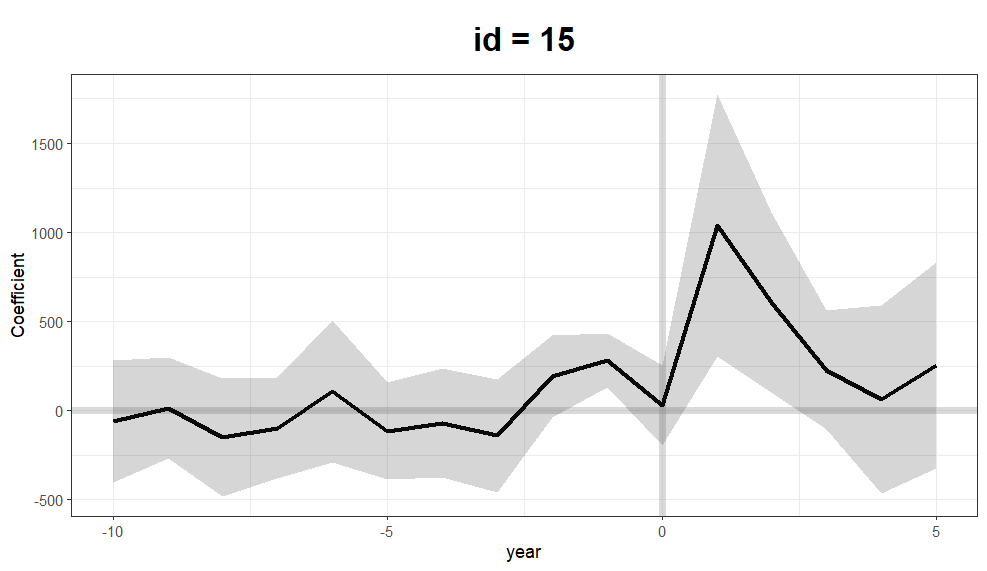
\includegraphics[width=\linewidth]{Main_Gap.png}
\end{minipage}
\hfill
\begin{minipage}{0.48\textwidth}
    \centering
    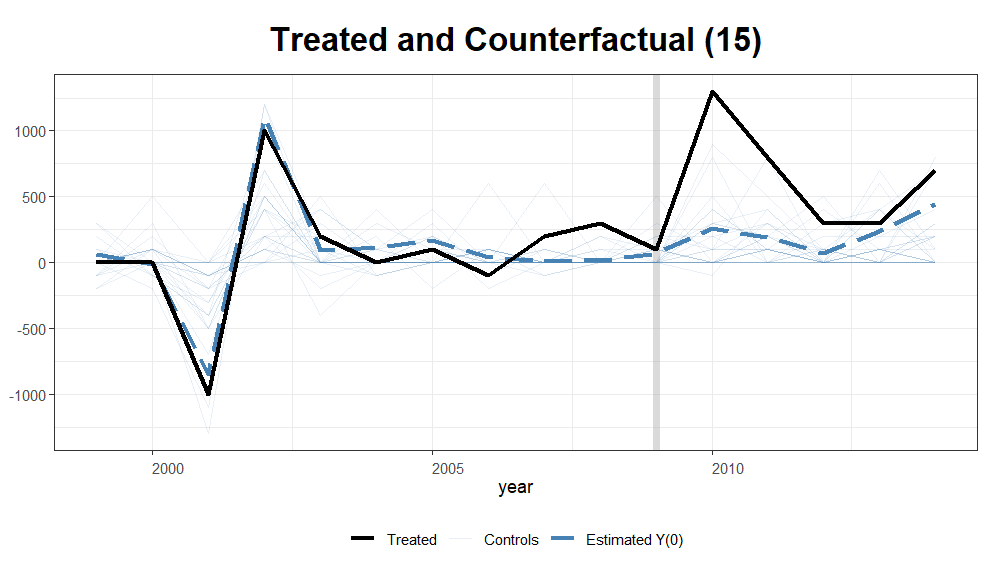
\includegraphics[width=\linewidth]{Main_Counterfactual.png}
\end{minipage}

\vspace{0.5cm}

\begin{minipage}{0.48\textwidth}
    \centering
    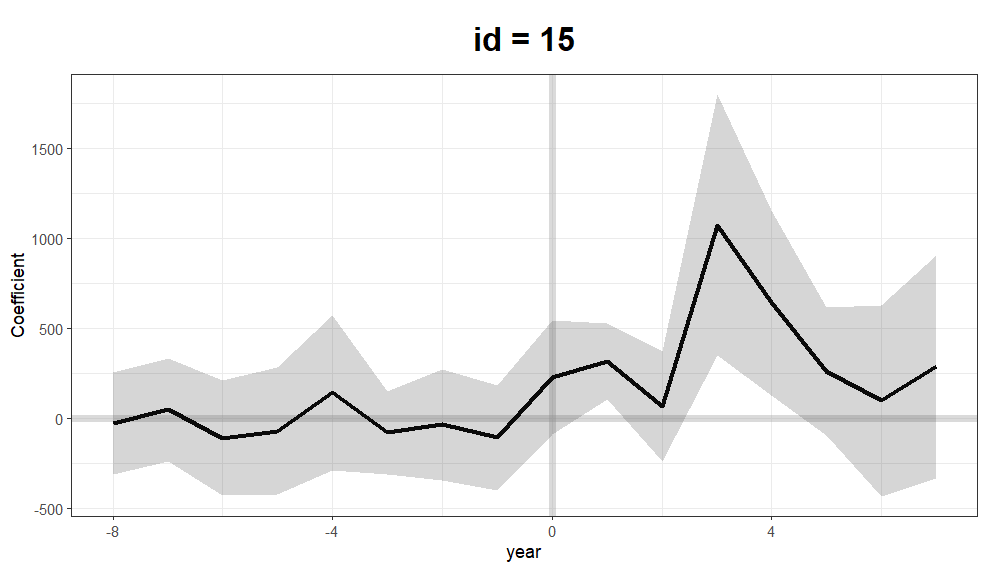
\includegraphics[width=\linewidth]{Placebo_2008_Gap.png}
\end{minipage}
\hfill
\begin{minipage}{0.48\textwidth}
    \centering
    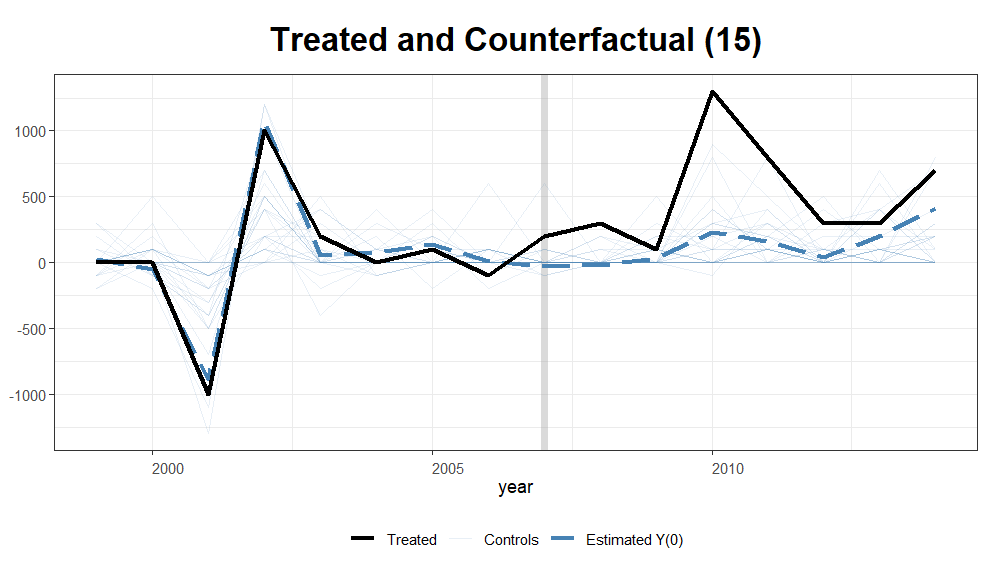
\includegraphics[width=\linewidth]{Placebo_2008_Counterfactual.png}
\end{minipage}

\caption{
Generalized synthetic control estimates for Inner Mongolia. 
Top left: estimated treatment effect (gap) with treatment beginning in 2010. 
Top right: treated and counterfactual trajectories under the main specification. 
Bottom left: estimated treatment effect under placebo treatment beginning in 2008. 
Bottom right: treated and counterfactual trajectories under the placebo specification.
}
\label{fig:gsc_panel}
\end{figure}

\section{Discussion}

My findings suggest that the Chinese state in 2010 was not revenue-maximizing, but rather resilience-maximizing-—prioritizing political stability legitimacy through public goods investment, even when investments in different provinces might have better maximized revenue. This case supports a more nuanced theory of public goods provision in which the state strategically deploys public goods as political instruments.

This has several implications. First, it may contribute to explanations of seemingly disproportionate public spending in regions that are politically sensitive, where the return on investment in fiscal terms may be low, but the return in stability and state or party consolidation is high. A productive line of research may be to evaluate the strength of this effect in democratic states, where dominant parties may prioritize public goods provision in electorally marginal districts. Second, this challenges whether we can simplify away political considerations in political economy models of the state, and specifically whether we can model public goods provision as endogenous to revenue-maximizing incentives. Third, this supports an extensive body of literature that identifies the pre-Xi Jinping Chinese state as one that pursued economic goals at least in part due to its legitimizing effects. Even now, attempts to influence Chinese policy through economic levers may have limited effects if the state values resilience more than fiscal performance.

\newpage

\section*{Appendix A: Comparative statics and proofs}

\subsection{Proof of Proposition \ref{prop:bindsonlyomega1}}

\begin{proof}
When \(\omega=1\), the state maximizes coercive slack directly:
\[
\max_{\tau,G} Z(\tau,G)
\]
subject to feasibility.

Consider an allocation \((\tau^*,G^*)\) satisfies
\[\label{eq:Ztaustar}
Z(\tau^*,G^*)=0.
\]

By assumption, there exists another feasible allocation \((\tau',G')\) such that
\[
Z(\tau',G')>0.
\]

Since the objective under pure resilience maximization is strictly increasing in \(Z\), it follows that
\[
Z(\tau',G') > Z(\tau^*,G^*).
\]

Therefore \((\tau^*,G^*)\) cannot be optimal, and in turn any optimal allocation under \(\omega=1\) must satisfy
\[
Z(\tau^*,G^*)>0,
\]
so the coercion constraint does not bind.
\end{proof}

\subsection{Proof of Proposition \ref{prop:pure_resilience}}

\begin{proof}
We first examine the objective function without considering the revenue constraint. Under $\omega=1$, holding inherited capacity $L$, fiscal capacity $F$, policy ambition $\Pi$, and expected shock environment fixed, the state maximizes
\[
Z(\tau,G)=\bar C_0 + \phi_G G + \phi_L L - C^R(\tau,G,F) - C^P(\Pi,L) - \E[C^S(\sigma,L)].
\]

Differentiating with respect to taxation gives
\[
\frac{\partial Z}{\partial \tau}=-C^R_\tau<0,
\]
since higher taxation increases coercive burden.

Differentiating with respect to public goods gives
\[
\frac{\partial Z}{\partial G}=\phi_G-C^R_G.
\]
Because $C^R_G<0$ and $\phi_G>0$, it follows that
\[
\frac{\partial Z}{\partial G}>0.
\]

Thus taxation lowers utility directly, while public goods raise utility directly.

Revenue therefore enters the problem only through the feasibility constraint:
\[
G+\Psi(C^{tot}) \le R^g(\tau,G,L,F,\varepsilon).
\]

Since taxation reduces the objective directly, the state chooses taxation only to the extent necessary to finance its preferred feasible allocation. Hence the pure resilience maximizer selects the minimum feasible tax rate, implying
\[
\tau^{rsl}\le \tau^{rev}.
\]

If a strictly lower feasible tax rate exists, the inequality is strict.
\end{proof}




\subsection{Proof of Proposition \ref{prop:tworegion_revenue_only}}

\begin{proof}
When $\omega=0$, the center solves
\[
\max_{G_A,G_B} \; N_A(G_A)+N_B(G_B)
\quad \text{s.t.} \quad G_A+G_B\le W.
\]
The Lagrangian is
\[
\mathcal L = N_A(G_A)+N_B(G_B)+\lambda(W-G_A-G_B).
\]
At an interior optimum,
\[
N_A'(G_A^*)=\lambda,\qquad N_B'(G_B^*)=\lambda,
\]
so
\[
N_A'(G_A^*)=N_B'(G_B^*).
\]
If the solution is not interior, the corresponding Kuhn--Tucker inequalities apply.

If at the relevant baseline $N_A'(G_A)<N_B'(G_B)$, then an additional unit of spending raises net fiscal return more in region $B$ than in region $A$. Therefore a pure revenue maximizer allocates marginal spending toward region $B$ until marginal returns are equalized or a corner is reached.
\end{proof}

\subsection{Proof of Proposition \ref{prop:tworegion_resilience_shift}}

\begin{proof}
When $\omega>0$, the center solves
\[
\max_{G_A,G_B}
\Big[
N_A(G_A)+N_B(G_B)+\omega\bigl(Z_A(G_A;\sigma_A,s_A)+Z_B(G_B;\sigma_B,s_B)\bigr)
\Big]
\]
subject to
\[
G_A+G_B\le W.
\]
The Lagrangian is
\[
\mathcal L=
N_A(G_A)+N_B(G_B)+\omega Z_A(G_A;\sigma_A,s_A)+\omega Z_B(G_B;\sigma_B,s_B)
+\lambda(W-G_A-G_B).
\]
At an interior optimum,
\[
N_A'(G_A^*)+\omega Z_{A,G}(G_A^*;\sigma_A,s_A)=\lambda,
\]
\[
N_B'(G_B^*)+\omega Z_{B,G}(G_B^*;\sigma_B,s_B)=\lambda.
\]
Hence
\[
N_A'(G_A^*)+\omega Z_{A,G}(G_A^*;\sigma_A,s_A)
=
N_B'(G_B^*)+\omega Z_{B,G}(G_B^*;\sigma_B,s_B).
\]

Relative to the revenue-only benchmark, spending shifts toward region $A$ whenever the added resilience term more than offsets $A$'s lower marginal fiscal return. Thus if
\[
Z_{A,G}(G_A;\sigma_A,s_A)>Z_{B,G}(G_B;\sigma_B,s_B)
\]
at the benchmark allocation, the resilience-weighted center allocates weakly more spending to region $A$ than would a pure revenue maximizer.
\end{proof}

\subsection{Proof of Proposition \ref{prop:tworegion_instability}}

\begin{proof}
Define
\[
F_A(G_A,G_B,\sigma_A,s_A,\lambda)
=
N_A'(G_A)+\omega Z_{A,G}(G_A;\sigma_A,s_A)-\lambda,
\]
\[
F_B(G_A,G_B,\lambda)
=
N_B'(G_B)+\omega Z_{B,G}(G_B;\sigma_B,s_B)-\lambda,
\]
together with the budget constraint
\[
G_A+G_B=W.
\]
At an interior optimum, these equations implicitly define $G_A^*$ and $G_B^*$.

Differentiating the first condition with respect to $\sigma_A$ gives
\[
\Big(N_A''(G_A^*)+\omega Z_{A,GG}(G_A^*;\sigma_A,s_A)\Big)\frac{dG_A^*}{d\sigma_A}
+\omega Z_{A,G\sigma}
-\frac{d\lambda}{d\sigma_A}
=0.
\]
Under the maintained second-order conditions, the own-effect term is negative. Since
\[
Z_{A,G\sigma}>0,
\]
an increase in $\sigma_A$ raises the marginal resilience payoff of expenditure in region $A$, which increases the optimal allocation to that region:
\[
\frac{dG_A^*}{d\sigma_A}>0.
\]

The same argument applies to $s_A$. Differentiating with respect to $s_A$ yields
\[
\Big(N_A''(G_A^*)+\omega Z_{A,GG}(G_A^*;\sigma_A,s_A)\Big)\frac{dG_A^*}{ds_A}
+\omega Z_{A,Gs}
-\frac{d\lambda}{ds_A}
=0.
\]
Because
\[
Z_{A,Gs}>0,
\]
a contemporaneous coercive shock raises the marginal resilience value of expenditure in region $A$, implying
\[
\frac{dG_A^*}{ds_A}>0.
\]
\end{proof}

\section{Appendix B: Revisions made for the MA Defense}

\subsubsection{Clarifying resilience vs. long-run survival}

I assert that resilience is a terminal value, and demonstrate that rulers who prioritize long-run survival value resilience under certain conditions. To do so, I briefly consider in \ref{section:resiliencedef} a dynamic model where the state cares about survival to the extent that it enables future revenue extraction, thus incorporating the coercion constraint dynamically. I explain that a state that cares about long-run survival cares about coercive slack only if it assesses itself to be near-collapse and is sufficiently risk-averse. Otherwise, it does not care about coercive slack as a terminal value.

\subsubsection{Limitations of my Synthetic Control Design}

I consider whether my sythetic control design can eliminate the below alternatives:
\begin{itemize}
    \item general budget expansion under the windfall,
    \item revenue-enhancing reinvestment in the windfall province itself,
    \item provincial-government capture of REE-linked revenue leading to locally funded spending.
\end{itemize}

The first two points relate to whether propositions \ref{prop:tworegion_revenue_only} and \ref{prop:tworegion_resilience_shift} actually map to the hypotheses $H_0$ and $H_1$. The key point that I clarify is that this mapping is valid because the process of revenue collection and expenditure in China is dominated by the central state. First, most of the revenue windfall should have gone to the state-owned enterprise that extracts and exports REEs of Inner Mongolia. Second, revenue captured by the provincial government is first redirected to the central government, who then re-allocates the aggregated revenue to provinces. Therefore, general budget expansion under the windfall cannot explain the evidence for $H_1$: although the central government does enjoy a growth in budget, this growth does not explain why the central government chooses to invest in a certain province. The synthetic control method naturally accounts for the growth in the outcome variable being a prevalent trend across all units. Likewise, revenue-enhancing reinvestment in the windfall province is certainly possible, but my theory indicates that the marginal value of revenue-enhancing reinvestment should be low compared to any number of other provinces with worse public goods. Thus a revenue-maximizing state should not be investing in Inner Mongolia to generate further revenue because the opportunity cost is higher than the revenue returns. While it is possible that the central government wanted to capture the anticipated growing demand in REEs by investing in Inner Mongolia, this should have led to a more persistent effect on rail construction, rather than the spike we see here.
The provincial-government capture of REE-linked revenue is implausible under the structure of the contemporary central-provincial fiscal relationship.  Moreover, revenue streams for the provincial government that are not directed to the central government should be controlled for by provincial expenditure in my SCM model.


\newpage

%% Use \bibliography{...} if using BibTeX
%TC:subst \printbibliography \bibliography
%TC:macro \field [0,1]
%TC:macro \name [0,0,0,1]
%TC:macro \list [0,0,1]
%% Use \printbibliography if using BibLaTeX

\printbibliography

\end{document}